\documentclass[10pt]{beamer}

\usepackage{amsmath}
\usepackage{amssymb}
\usepackage{amstext}

\title{Linear Algebra}

\author{Connor Briggs}


\begin{document}
\maketitle

\begin{frame}
  \frametitle{Linear Algebra}
  \begin{itemize}
  \item Linear algebra is the study of linear operators and linear equations.
  \item It often involves studying the behaviors of matrices and vectors, but its theorems can generalize well to other objects.
  \item The basic concepts are the vector space and the linear operator.
  \end{itemize}
\end{frame}

\begin{frame}
  \frametitle{Vector Spaces}
  A \textbf{vector space} $V$ over a field $F$ is a set equipped with two operators known as \textbf{vector addition} $+: V\times V\rightarrow V$ and \textbf{scalar multiplication} $*:F\times V\rightarrow V$ that obeys the following vector space axioms. Note that scalar multiplication is often indicated with juxtaposition.
  \begin{itemize}
  \item Closure under addition: $\forall_{\mathbf{u},\mathbf{v}\in V}\mathbf{u} + \mathbf{v} \in V$
  \item Closure under scalar multiplication: $\forall_{a\in F, \mathbf{v}\in V}a\mathbf{v} \in V$
  \item Associativity of vector addition: $\forall_{\mathbf{u},\mathbf{v},\mathbf{w}\in V} \mathbf{u} + (\mathbf{v} + \mathbf{w}) = (\mathbf{u} + \mathbf{v}) + \mathbf{w} = \mathbf{u} + \mathbf{v} + \mathbf{w}$
  \item Commutativity of Addition: $\forall_{\mathbf{u},\mathbf{v}\in V} \mathbf{u} + \mathbf{v} = \mathbf{v} + \mathbf{u}$
  \item Additive identity: $\exists_{\mathbf{0}\in V}\forall_{\mathbf{v}\in V}\mathbf{0} + \mathbf{v} = \mathbf{v}$
  \item Additive inverse: $\forall_{\mathbf{v}\in V}\exists_{-\mathbf{v}\in V}\mathbf{v} + (-\mathbf{v}) = \mathbf{0}$
  \item Compatibility of scalar multiplication: $\forall_{a,b\in F, \mathbf{v}\in V}a(b\mathbf{v}) = (ab)\mathbf{v}$
  \item Multiplicative identity: Since $F$ is a field, it contains an idenity element $1_F\in F$. $\forall_{\mathbf{v}\in V} 1_F\mathbf{v} = \mathbf{v}$.
  \item Right distributivity: $\forall_{a\in F,\mathbf{u}, \mathbf{v}\in V} a(\mathbf{u} + \mathbf{v}) = a\mathbf{u} + a\mathbf{v}$
  \item Left distributivity: $\forall_{a,b\in F, \mathbf{u}\in V}(a + b)\mathbf{u} = a\mathbf{u} + b\mathbf{u}$
    \end{itemize}
\end{frame}

\begin{frame}
  \frametitle{Vector Spaces}
  \begin{itemize}
  \item An element of a vector space is called a \textbf{vector}.
  \item An element of the field a vector space is based on is called a \textbf{scalar}.
  \item The definition of a field is given in the appendix, but is not necessary for this lecture. It is succficient to know that both $\mathbb{R}$ and $\mathbb{C}$ are fields, as is $\mathbb{Q}$, but $\mathbb{Z}$ and $\mathbb{N}$ are not.
  \item Common vector spaces include lists of real or complex numbers $\mathbb{R}^n$ and $\mathbb{C}^n$.
  \item However, it is possible to have an infinite dimensional vector space, such as the set of all real functions.
  \item When we write vectors, we often write them as a column of values. For instance, the following are real-valued vectors.
    $$\left[\begin{matrix}
    1\\
    2\\
    3\end{matrix}\right]\in \mathbb{R}^3, \left[\begin{matrix}
    10\\
    9\\
    8\\
    7\end{matrix}\right]\in \mathbb{R}^4,\left[5\right] \in\mathbb{R}^1\equiv \mathbb{R}$$
  \end{itemize}
\end{frame}

\begin{frame}
  \frametitle{Dual Vector Spaces}
  \begin{itemize}
  \item Given some vector space $V$ on some field $F$, the \textbf{dual vector space} $V^*$ is defined as a vector space containing all \textbf{linear maps} $\phi: V\rightarrow F$. The dual space is also a vector space.
  \item The concept of the dual space generalizes the concept of vector transpositions.
  \item The elements of the dual space are known as covectors.
  \item The action of a covector on a vector gives the dot product.
  \end{itemize}
  The covectors for the vectors on the previous slide are as follows.
  $$\left[\begin{matrix}
      1 & 2 & 3
    \end{matrix}\right] \in \mathbb{R}^{3*}, \left[\begin{matrix}
      10 & 9 & 8 & 7
    \end{matrix}\right] \in \mathbb{R}^{4*}, \left[5\right]\in \mathbb{R}^{1*} \equiv \mathbb{R}$$
  The \textbf{double-dual vector space} $V^{**}$ is technically not the original vector space. It is however isomorphic to the original vector space. This means that we can define a simple mapping onto the original vector space, and therefore we can treat the double-dual vector space as if it were the original vector space.
\end{frame}

\begin{frame}
  \frametitle{Dot Product}
  First, let's define a dot product. The dot product between two vectors is the sum of element-wise products. For instance, suppose we have the following two vectors.
  $$\mathbf{a} = \left[\begin{matrix}
      -4\\
      -6\\
      9\\
      -2
    \end{matrix}\right], \mathbf{b} = \left[\begin{matrix}
      -2\\
      1\\
      9\\
      3
    \end{matrix}\right]$$
  The dot product between these two vectors would be
  $$\mathbf{a}\cdot\mathbf{b} = (-4)(-2) + (-6)(1) + (9)(9) + (-2)(3) = 8 - 6 + 81 - 6 = 77$$

  As mentioned in the dual space slide, we can think of this as acting the dual of the first vector on the second.

  $$\left[\begin{matrix}
      -4 & -6 & 9 & -2
    \end{matrix}\right] \left[\begin{matrix}
      -2\\
      1\\
      9\\
      3
    \end{matrix}\right] = \mathbf{a}\cdot\mathbf{b} = 77$$
\end{frame}

\begin{frame}
  \frametitle{Basis Sets}
  A \textbf{basis} of a vector space $V$ is a set $B \subseteq V$ such that the following two axioms hold.
  \begin{itemize}
  \item Linear independence: For every finite subset $\left\{\mathbf{v}_1, \mathbf{v}_2, \cdots, \mathbf{v}_n\right\} \subseteq B$, if $\sum_{m=1}^{n}c_m\mathbf{v}_m = 0$ for some $c_1, c_2, \cdots, c_n \in F$, then $c_1 = c_2 = \cdots = c_n = 0$.
  \item Span: $\forall_{\mathbf{v}\in V}\exists_{a_1,a_2, \cdots, a_n\in F, \mathbf{v}_1, \mathbf{v}_2, \cdots, \mathbf{v}_n\in B} \sum_{m = 1}^na_m\mathbf{v}_m = \mathbf{v}$
  \end{itemize}
  Every vector space has a basis\footnote{This assumes the axiom of choice.}. Because of this, we can identify a vector space by its basis set. The operation of extending a basis to the entire vector space is called the \textbf{span}. For instance,
  $$\mathsf{Span}\left(\left\{\left[\begin{matrix}
      2\\
      1
    \end{matrix}\right], \left[\begin{matrix}
      1\\
      2
    \end{matrix}\right]\right\}\right) = \mathbb{R}^2$$

  The dimension of a vector space is the size of the smallest basis that spans it. That is,
  $$\mathsf{dim}(V) = \min_{B\subseteq V}\left(\left|B\right| : \mathsf{Span}(B) = V\right)$$
\end{frame}

\begin{frame}
  \frametitle{Linear Operators}
  A \textbf{linear operator} $M: V \rightarrow W$, where $V$ and $W$ are vector spaces that are based on the same scalar field $F$, is an operator that obeys the following axioms.
  \begin{itemize}
  \item Additivity: $\forall_{\mathbf{u}, \mathbf{v}\in V} M(\mathbf{u} + \mathbf{v}) = M(\mathbf{u}) + M(\mathbf{v})$
  \item Scalar multiplicity: $\forall_{a\in F, \mathbf{u}\in V}M(a\mathbf{u}) = aM(\mathbf{u})$
  \end{itemize}
  Note that if $W = F$, then $M$ is called a \textbf{linear form}. When dealing with finite vector spaces, we can prove that the only possible linear operators can be written as \textbf{matrices}. A matrix is a collection of numbers placed in a grid.
  $$\left[\begin{matrix}
      1 & 2\\
      3 & 4\\
      10 & 11
    \end{matrix}\right] \in \mathbb{R}^{2\times 3}$$
\end{frame}

\begin{frame}
  \frametitle{Matrix Subspaces}
  We can think of the rows and columns of a matrix as lists of vectors which form a basis for a vector space. These are called the \textbf{row space} and \textbf{column space} of a matrix. Consider the matrix from the previous slide. The row space is
  $$\mathsf{Span}\left(\left\{\left[\begin{matrix}
      1\\
      3\\
      10
    \end{matrix}\right], \left[\begin{matrix}
      2\\
      4\\
      11
    \end{matrix}\right]\right\}\right)$$
  and the column space is
  $$\mathsf{Span}\left(\left\{\left[\begin{matrix}
      1\\
      2
    \end{matrix}\right], \left[\begin{matrix}
      3\\
      4
    \end{matrix}\right], \left[\begin{matrix}
      10\\
      11
    \end{matrix}\right]\right\}\right)$$
\end{frame}

\begin{frame}
  \frametitle{Operator Arithmetic}
  We can define operations on our operators. Suppose we have two operators $A, B: V\rightarrow W$. We can define their sum as $\left(A + B\right)(\mathbf{v}) = A(\mathbf{v}) + B(\mathbf{v})$. We can also define the product of two operators. Let $C: V\rightarrow W$ and $D: W\rightarrow X$. Then $\left(CD\right)(\mathbf{v}) = C\left(D(\mathbf{v})\right)$. For matrices, the sum is fairly straightforward, being just a sum of the corresponding indices.
  $$\left[\begin{matrix}
      -3 & -4\\
      7 & -7
    \end{matrix}\right] + \left[\begin{matrix}
      -4 & -8\\
      2 & -3
    \end{matrix}\right] = \left[\begin{matrix}
      -7 & -12\\
      9 & -10
    \end{matrix}\right]$$
  Matrix multiplication is more complicated, but we can explain what is going on. First, break the left matrix up into row vectors and the right matrix into column vectors.
  $$\left[\begin{matrix}
      \left[\begin{matrix}
          -3 & -4\end{matrix}\right] \\
      \left[\begin{matrix}
          7 & -7\end{matrix}\right]\end{matrix}\right]\left[\begin{matrix}
      \left[\begin{matrix}
          -4\\
          2\end{matrix}\right] & \left[\begin{matrix}
          -8\\
          -3\end{matrix}\right]\end{matrix}\right]$$

  The result will be a new matrix whose entries are made up of dot products of the new vectors. The row index determines the covector from the left matrix, while the column index determines the vector from the right matrix.
      
\end{frame}

\begin{frame}
  \frametitle{Matrix Multiplication Worked}
  $$\left[\begin{matrix}
      -3 & -4\\
      7 & -7
    \end{matrix}\right] \left[\begin{matrix}
      -4 & -8\\
      2 & -3
    \end{matrix}\right]$$
  $$= \left[\begin{matrix}
      (-3)(-4) + (-4)(2) & (-3)(-8) + (-4)(-3)\\
      (7)(-4) + (-7)(2) & (7)(-8) + (-7)(-3)
    \end{matrix}\right]$$
  $$= \left[\begin{matrix}
      4 & 36\\
      -42 & -35
    \end{matrix}\right]$$
  Note that in order to perform matrix multiplication, the two matrices need to be compatible. If we have an $m \times n$ matrix and a $k \times l$ matrix, $n$ must equal $k$ before we can even think about multiplying the two matrices. Matrix multiplication is also not commutative. If we take the reverse of the multiplication above, we get
  $$\left[\begin{matrix}
      -4 & -8\\
      2 & -3
    \end{matrix}\right] \left[\begin{matrix}
      -3 & -4\\
      7 & -7
    \end{matrix}\right] = \left[\begin{matrix}
      -44 & 72\\
      -27 & 13\end{matrix}\right]$$
\end{frame}

\begin{frame}
  \frametitle{Matrix Transpose}
  Oftentimes, we need to switch our vector space to the dual space. If we want to have a matrix that operates the same way but on covectors, we need to find the \textbf{matrix transpose}. The matrix transpose is denoted by a superscript T, like $\mathbf{A}^T$. To get the matrix transpose, turn the rows of a matrix into the columns and vice versa.
  $$\left[\begin{matrix}
      -7 & 1\\
      -10 & 1\\
      -9 & 10
    \end{matrix}\right]^T = \left[\begin{matrix}
      -7 & -10 & -9\\
      1 & 1 & 10
    \end{matrix}\right]$$
  Due to how complex numbers work, we often care about the conjugate. This leads to the idea of the conjugate transpose. The way this works is you take the matrix, take its transpose, then take the complex conjugate of all of its elements.
\end{frame}

\begin{frame}
  \frametitle{Transpose Properties}
  \begin{itemize}
  \item If $\mathbf{A}^T = \mathbf{A}$, then we call $\mathbf{A}$ a \textbf{symmetric matrix}. The complex version of this is $\mathbf{A}^H = \mathbf{A}$, and we call this a \textbf{Hermitian matrix}.
  \item The rank of a matrix and its transpose are the same.
  \item The determinant and trace of a matrix and its transpose are the same.
  \item $\left(\mathbf{AB}\right)^T = \mathbf{B}^T\mathbf{A}^T$. Same applies to conjugate transpose.
  \item $\left(\mathbf{A} + \mathbf{B}\right)^T = \mathbf{A}^T + \mathbf{B}^T$
  \item $\left(x\mathbf{A}\right)^T = x\mathbf{A}^T$, but $\left(x\mathbf{A}\right)^H = x^*\mathbf{A}^H$
  \item If $\mathbf{A}^T = \mathbf{A}^{-1}$, we call $\mathbf{A}$ a \textbf{unitary matrix}.
  \end{itemize}
\end{frame}

\begin{frame}
  \frametitle{Systems of Linear Equations}
  We can represent a system of linear equations using matrices. Suppose we have the following system.
  $$-3x - 3y = 2$$
  $$3x - 9y = 2$$

  We can convert this into a matrix equation as follows.

  $$\left[\begin{matrix}
      -3 & -3\\
      3 & -9
    \end{matrix}\right]\left[\begin{matrix}
      x\\
      y\end{matrix}\right] = \left[\begin{matrix}
      2\\
      2\end{matrix}\right]$$

  We can solve the system using a process known as Gaussian elimination.
\end{frame}

\begin{frame}
  \frametitle{Gaussian Elimination}
  In Gaussian elimination, there are three basic operations we can perform.
  \begin{enumerate}
  \item We can swap any two rows in the coefficient matrix. Doing so also swaps the elements in the output matrix.
  \item We can scale any single row by any scalar. Doing so requires the corresponding element in the output to be scaled by the same amount.
  \item We can add any row to any other row. Again, we need to do the same thing to the output vector.
  \end{enumerate}

  The goal of Gaussian elimination is to achieve row-echelon form, where the first non-zero element in a row is 1 and the number of leading zeros increases down the matrix.
  $$\left[\begin{array}{cc|c}
      -3 & -3 & 2\\
      3 & -9 & 2
    \end{array}\right] \rightarrow \left[\begin{array}{cc|c}
      -3 & -3 & 2\\
      0 & -12 & 4
    \end{array}\right] \rightarrow \left[\begin{array}{cc|c}
      1 & 1 & -\frac{2}{3}\\
      0 & 1 & -\frac{1}{3}
    \end{array}\right]$$
\end{frame}

\begin{frame}
  \frametitle{Gaussian Elimination}
  We can take the result of Gaussian elimination to solve our equation.

  $$x + y = -\frac{2}{3}$$
  $$y = -\frac{1}{3} \rightarrow x = -\frac{1}{3}$$

  However, we can continue to perform the steps of Gaussian elimination. If we instead go until we have turned as many elements into zeros as possible, we reach a state known as \textbf{reduced row-echelon form}. The process becomes known as Gauss-Jordan elimination. If we take pick up the example from the previous step,
  $$\left[\begin{array}{cc|c}
      1 & 1 & -\frac{2}{3}\\
      0 & 1 & -\frac{1}{3}
    \end{array}\right]\rightarrow\left[\begin{array}{cc|c}
      1 & 0 & -\frac{1}{3}\\
      0 & 1 & -\frac{1}{3}
    \end{array}\right]$$
  This gives the following equations.

  $$x = -\frac{1}{3}$$
  $$y = -\frac{1}{3}$$
\end{frame}

\begin{frame}
  \frametitle{Rank}
  The example given above was a system of equations that could be solved. However, not all systems can be solved, and some systems have more equations than is necessary to determine the solution. The \textbf{rank} of a matrix can help us determine whether our system is overdetermined or underdetermined. In the case of Gaussian elimination, the rank of the matrix is simply the number of non-zero rows when the matrix is in row-echelon form. Formally, the rank is the number of dimensions of the row/column space. The two ways to determine this are equivalent, and the row-echelon form will actually give a reduced basis for the row/column space. The rank of an $n \times m$ matrix $A$ must satisfy $0 \le \mathsf{Rank}(A) \le \min(n, m)$. If $\mathsf{Rank}(A) = \min(n, m)$ and $n = m$, then the matrix is fully determined; if $n > m$, then the matrix is overdetermined. If $\mathsf{Rank}(A) < \min(n, m)$, then the matrix is underdetermined.
\end{frame}

\begin{frame}
  \frametitle{Determinant}
  The determinant of a square matrix tells us about how the matrix transforms a vector, and it can also tell us if the matrix is solvable. There are many ways to calculate the determinant. The easiest general way is to perform Gaussian elimination. Start with $\mathsf{det}(A)_0 = 1$. Whenever you swap two rows, $\mathsf{det}(A)_{n + 1} = -\mathsf{det}(A)_n$. Whenever you scale a row by some value $k$, $\mathsf{det}(A)_{n + 1} = k\mathsf{det}(A)_n$. Whenever you add one row to another, make no change to the determinant. When the matrix is in row-echelon form, look for any diagonal entries that are zero. If there are zeros on the diagonal, then the determinant is zero. Otherwise, the determinant is the value that you calculated.
\end{frame}

\begin{frame}
  \frametitle{Determinant}
  In the $2\times 2$ and $3\times 3$ cases, there are easier ways of calculating the determinant.
  \begin{center}
    
\includegraphics[width=0.08\textwidth]{2by2.png}
  \end{center}
  $$\mathsf{det}\left(\left[\begin{matrix}
      a & b\\
      c & d
    \end{matrix}\right]\right) = ad - bc$$
    \begin{center}
      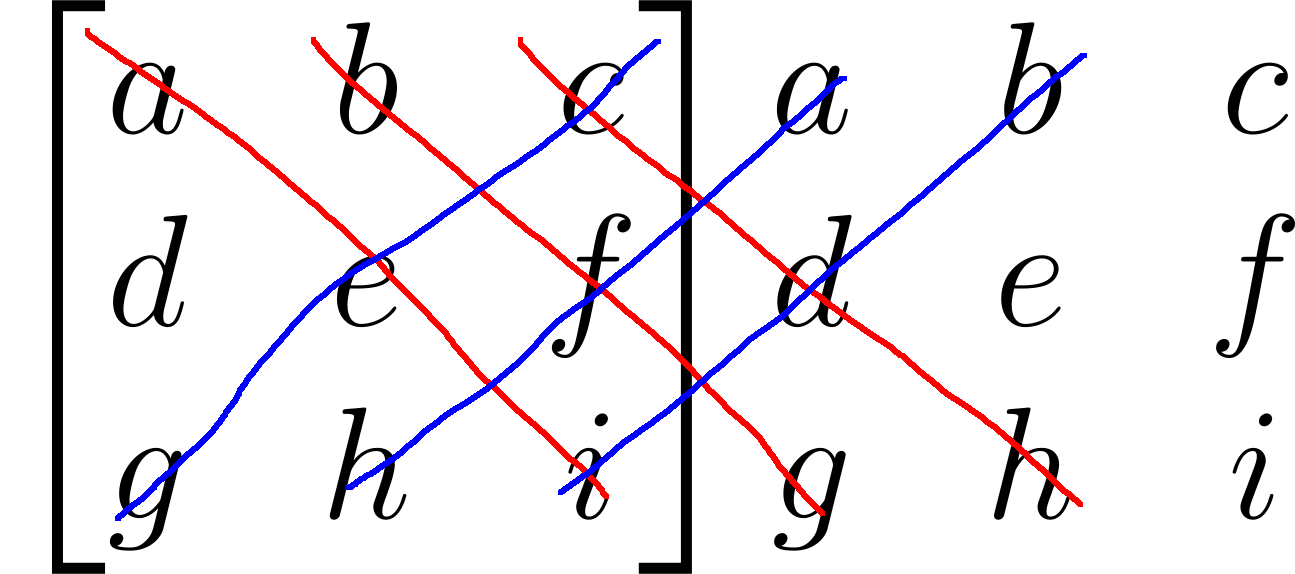
\includegraphics[width=0.25\textwidth]{3by3.png}
    \end{center}
    $$\mathsf{det}\left(\left[\begin{matrix}
a & b & c\\
d & e & f\\
g & h & i\end{matrix}\right]\right) = aei + bfg + cdh - ceg - afh - bdi$$

    This pattern does not generalize to higher dimensions.
\end{frame}

\begin{frame}
  \frametitle{Determinant}
  The determinant tells us how it scales space. A matrix with determinant of 2 would double the volume of an object. A matrix with a determinant of 0 is called a singular matrix. A singular matrix is one which can not be reduced, and the system of equations that it represents can not be solved.
\end{frame}

\begin{frame}
  \frametitle{Identity Matrix}
  The \textbf{identity matrix} is a square matrix that does not change the vector that it is operated on. Every element in the identity matrix is zero, except for the diagonal entries, which are all 1. For instance, the $4\times 4$ identity matrix is
  $$I_4 = \left[\begin{matrix}
      1 & 0 & 0 & 0\\
      0 & 1 & 0 & 0\\
      0 & 0 & 1 & 0\\
      0 & 0 & 0 & 1
    \end{matrix}\right]$$
\end{frame}

\begin{frame}
  \frametitle{Matrix Inverse}
  The \textbf{inverse} of a matrix $\mathbf{A}$ is the matrix $\mathbf{A}^{-1}$ that satisfies $\mathbf{AA}^{-1} = \mathbf{A}^{-1}\mathbf{A} = \mathbf{I}$. One easy way to solve for the inverse is to again use Gaussian elimination. On the left side of the bar, put the entries of the matrix $\mathbf{A}$. On the right, put the identity matrix, $\mathbf{I}$. Then, solve until you reach reduced row-echelon form. The left side should be the identity after this, and the right side will be the inverse of the input. If the left is not the identity, then the input matrix does not have an inverse. That is, the matrix is singular. For instance,
  $$\left[\begin{array}{ccc|ccc}
      -8 & -10 & -8 & 1 & 0 & 0\\
      -3 & 3 & -1 & 0 & 1 & 0\\
      -3 & 1 & 1 & 0 & 0 & 1
    \end{array}\right] \rightarrow \left[\begin{array}{ccc|ccc}
      1 & \frac{5}{4} & 1 & -\frac{1}{8} & 0 & 0\\
      -3 & 3 & -1 & 0 & 1 & 0\\
      -3 & 1 & 1 & 0 & 0 & 1
    \end{array}\right]$$
\end{frame}

\begin{frame}
  \frametitle{Inverse Worked}
  $$\rightarrow\left[\begin{array}{ccc|ccc}
      1 & \frac{5}{4} & 1 & -\frac{1}{8} & 0 & 0\\
      0 & \frac{27}{4} & 2 & -\frac{3}{8} & 1 & 0\\
      0 & \frac{19}{4} & 4 & -\frac{3}{8} & 0 & 1
    \end{array}\right] \rightarrow \left[\begin{array}{ccc|ccc}
      1 & \frac{5}{4} & 1 & -\frac{1}{8} & 0 & 0\\
      0 & 1 & \frac{8}{27} & -\frac{1}{18} & \frac{4}{27} & 0\\
      0 & 1 & \frac{16}{19} & -\frac{3}{38} & 0 & \frac{4}{19}
    \end{array}\right]$$
  $$\rightarrow\left[\begin{array}{ccc|ccc}
      1 & 0 & \frac{17}{27} & -\frac{1}{18} & -\frac{5}{27} & 0\\
      0 & 1 & \frac{8}{27} & -\frac{1}{18} & \frac{4}{27} & 0\\
      0 & 0 & \frac{280}{513} & -\frac{4}{171} & -\frac{4}{27} & \frac{4}{19}
    \end{array}\right] \rightarrow \left[\begin{array}{ccc|ccc}
      1 & 0 & \frac{17}{27} & -\frac{1}{18} & -\frac{5}{27} & 0\\
      0 & 1 & \frac{8}{27} & -\frac{1}{18} & \frac{4}{27} & 0\\
      0 & 0 & 1 & -\frac{3}{70} & -\frac{19}{70} & \frac{27}{70}
    \end{array}\right]$$
  $$\rightarrow\left[\begin{array}{ccc|ccc}
      1 & 0 & 0 & -\frac{1}{35} & -\frac{1}{70} & -\frac{17}{70}\\
      0 & 1 & 0 & -\frac{3}{70} & \frac{8}{35} & -\frac{4}{35}\\
      0 & 0 & 1 & -\frac{3}{70} & -\frac{19}{70} & \frac{27}{70}
    \end{array}\right]$$
\end{frame}

\begin{frame}
  \frametitle{Check our Work}

  If we multiply the matrix we found by the starting matrix, we should get the identity.

  $$\left[\begin{matrix}
      -8 & -10 & -8\\
      -3 & 3 & -1\\
      -3 & 1 & 1
    \end{matrix}\right]\left[\begin{matrix}
      -\frac{2}{70} & -\frac{1}{70} & -\frac{17}{70}\\
      -\frac{3}{70} & \frac{16}{70} & -\frac{8}{70}\\
      -\frac{3}{70} & -\frac{19}{70} & \frac{27}{70}
    \end{matrix}\right]$$

  $$\left[\begin{matrix}
      \frac{16 + 30 + 24}{70} & \frac{8 - 160 + 152}{70} & \frac{136 + 80 - 216}{70}\\
      \frac{6 - 9 + 3}{70} & \frac{3 + 48 + 19}{70} & \frac{51 - 24 - 27}{70}\\
      \frac{6 - 3 - 3}{70} & \frac{3 + 16 - 19}{70} & \frac{51 - 8 + 27}{70}
    \end{matrix}\right] = \left[\begin{matrix}
      1 & 0 & 0\\
      0 & 1 & 0\\
      0 & 0 & 1
    \end{matrix}\right]$$
  As expected.
\end{frame}

\begin{frame}
  \frametitle{Kernel or Nullspace}
  The \textbf{kernel} or \textbf{nullspace} of a linear operator (like a matrix) is the set of all inputs that yield the zero vector. That is, $\mathsf{ker}(A) = \left\{\mathbf{x} : A(\mathbf{x}) = \mathbf{0}\right\}$. We can find the nullspace by simply performing Gauss-Jordan elimination. A basis for the nullspace is the set of column vectors in the matrix that have a zero on the diagonal.
\end{frame}

\begin{frame}
  \frametitle{Eigenvalue Equations}
  Very often, we want to solve an equation that looks like this.
  $$\mathbf{Av} = \lambda\mathbf{v}$$
  We call this kind of equation an \textbf{eigenvalue equation}. Here, $\lambda$ is called an \textbf{eigenvalue} of $\mathbf{A}$ and $\mathbf{v}$ is called an \textbf{eigenvector} of $\mathbf{A}$. Only square matrices can have eigenvalues, and a general linear operator needs to output into the same space as its input. That is, $\phi: V \rightarrow V$. Eigenvalues can appear multiple times for a matrix, something deemed \textbf{multiplicity} or \textbf{degeneracy}. To solve for the eigenvalues, we can first calculate the \textbf{characteristic polynomial} in $\lambda$ as follows.
  $$\mathsf{det}\left(\mathbf{A} - \lambda\mathbf{I}\right) = \mathbf{0}$$
  The solutions to this characteristic equation are the eigenvalues of the matrix $\mathbf{A}$. Note that $\mathbf{I}$ is the identity matrix with the same dimensions as $\mathbf{A}$.
\end{frame}

\begin{frame}
  \frametitle{Eigenvectors}
  From here, we can find the eigenvectors. To do this, we can solve the following equation for the $k$th eigenvalue.
  $$\left(\mathbf{A} - \lambda_k\mathbf{I}\right)\mathbf{v}_k = \mathbf{0}$$

  Note that the degeneracy of $\lambda_k$ in the characteristic polynomial (\textbf{algebraic multiplicity}) is not necessarily the same as the number of eigenvectors (\textbf{geometric multiplicity}) we obtain from this system of equations. If the two multiplicities are different, then the matrix is not \textbf{diagonalizable}.
\end{frame}

\begin{frame}
  \frametitle{Eigenvalue Properties}
  \begin{itemize}
  \item For some matrix $\mathbf{A}$ with eigenvalues $\lambda_k$ and algebraic multiplicities $n_k$, the product of the eigenvalues gives the determinant. $\prod_k\lambda_k^{n_k} = \mathsf{det}\left(\mathbf{A}\right)$.
  \item While we haven't mentioned the trace yet, the sum of the eigenvalues is also equal to the trace, or the sum of the diagonal entries of $\mathbf{A}$. $\sum_k n_k\lambda_{k} = \mathsf{Tr}\left(\mathbf{A}\right)$.
  \item If the input matrix is symmetric, then its eigenvalues are real. This also applies to the complex analog of symmetric matrices, known as Hermitian matrices.
  \item Given some invertible matrix $B$, if $\mathbf{A}$ is diagonalizable, then the eigenvalues of $\mathbf{BAB}^{-1}$ are the same as the eigenvalues of $\mathbf{A}$.
    \item The eigenvalues of $\mathbf{A}$ are the same as for $\mathbf{A}^T$.
  \end{itemize}
\end{frame}

\begin{frame}
  \frametitle{Eigendecomposition}
  If the algebraic multiplicities and geometric multiplicities of the eigenvalues of some matrix $\mathbf{A}$ match up with each other, then the matrix is diagonalizable. This means that we can write $\mathbf{A} = \mathbf{PDP}^{-1}$, where raising a matrix to the -1 is called the inverse, the columns of $\mathbf{P}$ are the eigenvectors of $\mathbf{A}$, and $\mathbf{D}$ is a matrix where all elements are zero, but the diagonal entries are the eigenvalues of $\mathbf{A}$.
\end{frame}

\begin{frame}
  \frametitle{Inner Product Spaces}
  An \textbf{inner product space} is a vector space $V$ over a field $F$, where $F$ must either be $\mathbb{R}$ or $\mathbb{C}$, together with an \textbf{inner product} $\left<\cdot, \cdot\right>: V\times V\rightarrow F$ such that the following axioms hold.
  \begin{itemize}
  \item Conjugate\footnote{If real, this is just symmetry} symmetry: $\forall_{\mathbf{u}, \mathbf{v}\in V}\left<\mathbf{u}, \mathbf{v}\right> = \left<\mathbf{v}, \mathbf{u}\right>^*$
  \item Linearity in the second argument\footnote{Physicist notation. Math notation has linearity in the first argument.}: $\forall_{a\in F, \mathbf{u}, \mathbf{v}\in V}\left<\mathbf{u}, a\mathbf{v}\right> = a\left<\mathbf{u}, \mathbf{v}\right>$, $\forall_{\mathbf{u}, \mathbf{v}, \mathbf{w}\in V}\left<\mathbf{u}, \mathbf{v} + \mathbf{w}\right> = \left<\mathbf{u}, \mathbf{v}\right> + \left<\mathbf{u}, \mathbf{w}\right>$
  \item Positive-definiteness: $\forall_{\mathbf{u}\in V, \mathbf{u}\ne \mathbf{0}}\left<\mathbf{u}, \mathbf{u}\right> > 0$
  \end{itemize}

  A very common example of an inner product is the dot product. Every inner product space also induces something called a norm. The \textbf{norm} $\left|\left|\cdot\right|\right|: V\rightarrow F$ induced by the inner product is given as $\left|\left|\mathbf{v}\right|\right| = \sqrt{\left<\mathbf{v}, \mathbf{v}\right>}$. Another way of representing the inner product is through bra-ket notation. Here, $\left<f\middle|g\right>$ is the same as $\left<f, g\right>$, and $\left<f\middle|\hat{\Omega}\middle|g\right>$ is the same as $\left<f, \hat{\Omega}g\right>$.
\end{frame}

\begin{frame}
  \frametitle{Graham-Schmidt Orthonormalization}
  If we are given some set of elements from an inner product space, we can perform orthonormalization on them. Two vectors $\mathbf{u}, \mathbf{v}\in V$ are \textbf{orthogonal} if $\left<\mathbf{u}, \mathbf{v}\right> = 0$, and $\mathbf{u}$ is \textbf{normal} if $\left<\mathbf{u}, \mathbf{u}\right> = 1$. Suppose we are given $u_1, u_2, \cdots, u_n \in V$. We can create a set of orthonormal vectors $v_1, v_2, \cdots v_n \in V$ by doing the following.
  \begin{enumerate}
  \item Start by setting $v_1 = \frac{u_1}{\left|\left|u_1\right|\right|}$.
  \item For the $k$th vector, we can find a new vector $\tilde{u}_k$ that is orthogonal to all previous vectors by taking $\tilde{u}_k = u_k - \sum_{i = 1}^{k - 1}\left<v_i, u_k\right> v_i$.
  \item We can take this orthogonal vector and normalize it to get the orthonormal vector, $v_k = \frac{\tilde{u}_k}{\left|\left|\tilde{u}_k\right|\right|}$.
  \end{enumerate}
\end{frame}

\begin{frame}
  \frametitle{Practice Problems}
  Here are some practice problems. Some of these are statements given before, which you should be able to prove.
  \begin{enumerate}
  \item Suppose we have the set $\mathbb{R}^2$ with addition defined as $\left[\begin{matrix}
      a\\
      b
    \end{matrix}\right] + \left[\begin{matrix}
      c\\
      d
    \end{matrix}\right] = \left[\begin{matrix}
      \frac{a + b}{2}\\
      \frac{c + d}{2}
    \end{matrix}\right]$ and scalar multiplication defined in the usual way. Does this constitute a vector space?
  \item Is the set of $2\times 2$ matrices, $\mathbb{R}^{2\times 2}$, with matrix addition and scalar-matrix multiplication a vector space?
  \item Using Gaussian elimination, find a basis for the column space of the matrix
    $$\left[\begin{matrix}
      -2 & -2 & 5 & -4\\
      -3 & 1 & 4 & -7\\
      -7 & -5 & 6 & -1\\
      5 & 3 & -1 & -3
    \end{matrix}\right]$$
    What is the dimensionality of the column space? Can you also give a basis for the nullspace?
  \end{enumerate}
\end{frame}
\begin{frame}
  \frametitle{Practice Problems}
  \begin{enumerate}
  \item Compute the following matrix product.
    $$\mathbf{A} = \left[\begin{matrix}
      2 & 1\\
      2 & 8\\
      1 & -1
    \end{matrix}\right], \mathbf{B} = \left[\begin{matrix}
      6 & 0\\
      8 & 9
    \end{matrix}\right], \mathbf{AB} = ?$$
    Are you able to compute $\mathbf{BA}$? If so, what is the product. If not, why not.
  \item For those same two matrices, show that $\left(\mathbf{AB}\right)^T = \mathbf{B}^T\mathbf{A}^T$.
  \item Find the determinant, and if possible the inverse, of the following matrix. If it's not possible to find the inverse, why not?
    $$\left[\begin{matrix}
      4 & 0 & 5\\
      10 & 3 & 10\\
      1 & -2 & 0
    \end{matrix}\right]$$
  \item Find the characteristic polynomial for the above matrix. You do not have to solve it.
  \item Find the eigenvalues and eigenvectors of the following matrix.
    $$\left[\begin{matrix}
      0 & 5\\
      -3 & 1
    \end{matrix}\right]$$
  \end{enumerate}
\end{frame}
\begin{frame}
  \frametitle{Practice Problems}
  \begin{enumerate}
  \item Prove: Given some invertible matrix $\mathbf{B}$, if $\mathbf{A}$ is diagonalizable, then the eigenvalues of $\mathbf{BAB}^{-1}$ are the same as the eigenvalues of $\mathbf{A}$.
  \item Prove that the dot product on $\mathbb{R}^n$ constitutes an inner product.
  \item Prove that $\left<f, g\right> = \int_{-\infty}^{\infty} f^*(x)g(x)\mathsf{d}x$ constitutes an inner product.
  \item Using the fact that $\mathsf{det}(\mathbf{AB}) = \mathsf{det}(\mathbf{A})\mathsf{det}(\mathbf{B})$, show that for some invertible matrix $\mathbf{A}$, $\mathsf{det}(\mathbf{A}^{-1}) = \frac{1}{\mathsf{det}(\mathbf{A})}$
  \item Prove the Cauchy-Schwarz inequality, without assuming the triangle inequality. That is, for some inner product and its induced norm, $\left|\left<x, y\right>\right| \le \left|\left|x\right|\right|\left|\left|y\right|\right|$.
  \item Assuming the Cauchy-Schwartz inequality holds, prove the triangle inequality in general. That is, for some norm induced by an inner product, $\left|\left|x + y\right|\right| \le \left|\left|x\right|\right| + \left|\left|y\right|\right|$.
  \end{enumerate}
\end{frame}
\begin{frame}
  \frametitle{Practice Problems}
  \begin{enumerate}
  \item By defining the concept of a dual vector space, we defined a way to construct dot products. However, the axioms of the dual vector space do not imply an inner product. Why might this be the case? Could you construct a vector space and its dual such that the action of a covector does not constitute an inner product?
  \item The $n$th Fibonacci number can be found using matrix powers (described in the appendix) as follows.
    $$\left[\begin{matrix}
      1 & 1\\
      1 & 0
    \end{matrix}\right]^n\left[\begin{matrix}
      0\\
      1
    \end{matrix}\right] = \left[\begin{matrix}
      F_n\\
      F_{n - 1}
    \end{matrix}\right]$$
    Derive Binet's formula, $F_n = \frac{\phi^n - (-\phi)^{-n}}{\sqrt{5}}$, where $\phi = \frac{1 + \sqrt{5}}{2}, \phi^2 = \phi + 1, \frac{1}{\phi} = \phi - 1$.
  \end{enumerate}
\end{frame}

\begin{frame}
  \frametitle{Appendix: Fields}
  A \textbf{field} F is a set along with two operations, multiplication and addition, $*: F\times F\rightarrow F$ and $+: F\times F\rightarrow F$ such that the following axioms are satisfied.
  \begin{itemize}
  \item Closure: $\forall_{a,b\in F}a + b\in F$ (monoid)
  \item Associativity: $\forall_{a,b,c\in F} a + (b + c) = (a + b) + c = a + b + c$ (monoid)
  \item Identity: $\exists_{0_F\in F}\forall_{a\in F} a + 0_F = 0_F + a = a$ (monoid)
  \item Solvability: $\forall_{a\in F}\exists_{-a\in F}a + (-a) = (-a) + a = 0_F$ (group)
  \item Commutativity: $\forall_{a, b\in F} a + b = b + a$ (Abelian group)
  \item $\left<F, *\right>$ is a monoid. The multiplicative identity is known as $1_F$. (ring)
  \item Distributivity: $\forall_{a, b, c \in F}a (b + c) = ab + ac \wedge (a + b)c = ac + bc$ (ring)
    \item Commutativity: $\forall_{a, b\in F} ab = ba$ (commutative ring)
    \item No zero divisors: $\forall_{a, b\in F} ab = 0 \rightarrow a = 0 \vee b = 0$ (integral domain)
    \item Divisibility: $\forall_{a\in F, a \ne 0_F} \exists_{b\in F} ab = 1_F$ (field)
  \end{itemize}
\end{frame}

\begin{frame}
  \frametitle{QR Decomposition}
  The Graham-Schmidt procedure, outlined previously, induces a nice way of decomposing a matrix. Let $\mathbf{A}$ be an $n\times m$ matrix. We can orthonormalize the column space of $\mathbf{A}$ to get two matrices, which we will call $\mathbf{Q}$ and $\mathbf{R}$. The columns of $\mathbf{Q}$ will simply be the orthonormal vectors that we get out of the Graham-Schmidt procedure. Meanwhile, $\mathbf{R}$ will be an $m \times m$ matrix, where $R_{ij} = \left<v_i, u_j\right>$ if $i < j$, $R_{ij} = \left|\left|\tilde{u}_k\right|\right|$ if $i = j$, and $R_{ij} = 0$ if $i > j$. $\mathbf{R}$ should be upper-triangular, or in row-echelon form. This decomposition lets us write $\mathbf{A} = \mathbf{QR}$.

  There is an excellent algorithm for computing the eigenvalues and eigenvectors of a matrix called the QR algorithm. The way to do it is to start with $\mathbf{A}_0 = \mathbf{A}$. Then, at step $k$, write $\mathbf{A}_{k} = \mathbf{QR}$. To get the next guess, simply swap the matrices. That is, $\mathbf{A}_{k + 1} = \mathbf{RQ}$. If you keep doing this, you end up with a diagonally dominant matrix, and the diagonal entries will approach the eigenvalues of $\mathbf{A}$. In real applications, some preconditioning will be applied to $\mathbf{A}$ to improve the speed of the algorithm. (excercise: use the fact that $\mathbf{Q}$ is invertible to show that the eigenvalues of $\mathbf{A}_k$ are the same as for $\mathbf{A}$. Note also that $\mathbf{Q}^H = \mathbf{Q}^{-1}$.)
\end{frame}

\begin{frame}
  \frametitle{Hilbert Spaces}
  A \textbf{Hilbert space} is a set of square-integrable functions. The solutions to the Schrödinger equation for any potential belong to a Hilbert space. The basis to the free-particle Hilbert space is $\left\{\delta(\mathbf{r} + \mathbf{y}): \mathbf{y} \in \mathbb{R}^3\right\}$, that is, the Dirac delta functions centered at all coordinates. Other potentials have different basis sets. For instance, the particle in a 1d box has a basis of $\left\{\sqrt{\frac{2}{L}}\sin\left(\frac{n\pi x}{L}\right) : n \in \mathbb{N}\right\}$. Hilbert spaces are inner product spaces, which are also vector spaces. The vectors in a Hilbert space are functions. The inner product is represented as $\left<f, g\right> = \int_Vf(x)^*g(x)\mathrm{d}x$, where $V$ is the region over which the members of the Hilbert space are defined. The inner product here can also be represented by $\left<f\middle|g\right>$, which is known as bra-ket notation.
\end{frame}

\begin{frame}
  \frametitle{Function Application}
  Given a square matrix, $\mathbf{A}$, we can raise it to any positive integer power by multiplying it by itself that many times. $\mathbf{A}^4 = \mathbf{AAAA}$. If $A$ is invertible, we can also raise it to a negative power by exponentiating its inverse. $\mathbf{A}^{-4} = \mathbf{A}^{-1}\mathbf{A}^{-1}\mathbf{A}^{-1}\mathbf{A}^{-1}$. Now, let's suppose $\mathbf{A}$ is diagonalizable, with $\mathbf{A} = \mathbf{PDP}^{-1}$. Let's see what happens if we square $\mathbf{A}$.
  $$\mathbf{A}^2 = \mathbf{AA} = \mathbf{PDP}^{-1}\mathbf{PDP}^{-1} = \mathbf{PDDP}^{-1} = \mathbf{PD}^2\mathbf{P}^{-1}$$
  This extends to any integer power of $\mathbf{A}$ (try to prove that $\mathbf{A}^{-1}$ is the same as the inverse). Let's suppose we have some analytic function $f$ represented by the Taylor series $f(x) = \sum_{k = 0}^{\infty} \frac{a_kx^k}{k!}$. We can see what happens when we apply this Taylor series to our diagonalizable matrix.

  $$f(\mathbf{A}) = \sum_{k = 0}^{\infty} \frac{a_k\mathbf{A}^k}{k!} = \sum_{k = 0}^\infty \frac{a_k\mathbf{PD}^k\mathbf{P}^{-1}}{k!} = \mathbf{P}\left(\sum_{k = 0}^\infty\frac{a_k\mathbf{D}^k}{k!}\right)\mathbf{P}^{-1}$$
\end{frame}
\begin{frame}
  \frametitle{Function Application}
  Since $\mathbf{D}$ is a diagonal matrix, raising it to a power is the same as raising its diagonal entries to a power.

  $$\mathbf{D}^k = \left[\begin{matrix}
      \lambda_1^k & 0 & \cdots & 0\\
      0 & \lambda_2^k & \cdots & 0\\
      \vdots & \vdots & \ddots & \vdots\\
      0 & 0 & \cdots & \lambda_n^k
    \end{matrix}\right]$$
  It should also be fairly clear that adding together diagonal matrices will just give another diagonal matrix. Ultimately, what we end up with is the following.
  $$\left[\begin{matrix}
      f(\lambda_1) & 0 & \cdots & 0\\
      0 & f(\lambda_2) & \cdots & 0\\
      \vdots & \vdots & \ddots & \vdots\\
      0 & 0 & \cdots & f(\lambda_n)
    \end{matrix}\right]$$
  Let's call this $f(\mathbf{D})$. That is, applying an analytic function to a diagonal matrix is the same as applying the function to each of its diagonal elements.
\end{frame}

\begin{frame}
  \frametitle{Function Application}
  Now that we have a way of writing the inner sum, we can finally finish this construction.
  $$f(\mathbf{A}) = \mathbf{P}\left(\sum_{k=0}^\infty\frac{a_k\mathbf{D}^k}{k!}\right)\mathbf{P}^{-1} = \mathbf{P}f(\mathbf{D})\mathbf{P}^{-1}$$
  Some good examples of functions that we can use this with include $e^x$, $\log(x)$, $\sin(x)$, $x^n$, and more. Of course, we should note that any constant term $a_0$ will necessarily become $a_0\mathbf{I}$ when it is added to our matrices. Also, if we aren't worried about doing pure math with these things, we can also generalize our construction to include any function, not just analytic functions.
\end{frame}

\begin{frame}
  \frametitle{Multilinear Algebra}
  So far, we have discussed linear algebra. However, we often also deal with something called multilinear algebra. The basic concept in multilinear algebra is the tensor. A tensor is something that transforms like a tensor (yes, I know it's a bad definition, but it's the actual definition). That is, a \textbf{tensor} is an element of a tensor product space. A \textbf{tensor product} between two vector spaces $V\otimes W$ over the same field $F$ is defined as the vector space $V \otimes W$ along with the bilinear map $\phi: V\times W \rightarrow V\otimes W$ such that for all morphisms $h:V\times W\rightarrow Z$, there exists some morphism $\tilde{h}:V\otimes W\rightarrow Z$ such that $h = \tilde{h} \circ \phi$. That is, for all $v\in V$ and $w\in W$, $h(v, w) = \tilde{h}(\phi(v, w))$.
\end{frame}

\begin{frame}
  \frametitle{Multilinear Algebra}
  As a result of this definition, we can actually say a few things about this.
  \begin{itemize}
  \item If $V \ne W$, then $V \otimes W \equiv W \otimes V$. This means that if we are mapping between different spaces, the order of the mapping can be freely varied. If the spaces are the same, then this is not the case.
    \begin{itemize}
    \item If we consider the $T_2$ amplitudes, this is saying that for $t_{ij}^{ab}$, we can apply either $a$ and $b$ first, or $i$ and $j$ first, but we can't swap $a$ with $b$ or $i$ with $j$. In fact, doing so induces a sign change in this case.
    \end{itemize}
    \item The tensor product is associative, even if there are equivalent spaces in the product. This means that we don't need to care about the grouping of the products.
    \item The tensor product space is generated by a basis if the input spaces have bases. Suppose we have $B_W = \left\{e_1, e_2, \cdots, e_n\right\}$ and $B_V = \left\{e^1, e^2, \cdots, e^m\right\}$. The tensor product $V \otimes W$ will be generated by $B_{V\otimes W} = \left\{\left(e^i, e_j\right)\middle| 1 \le i \le m, 1 \le j \le n\right\}$. 
  \end{itemize}
\end{frame}

\begin{frame}
  \frametitle{Tensor Elements}
  The elements of a tensor can be accessed by applying the tensor to the list of covectors to its vector spaces. For instance, given some tensor $T \in V\otimes W$, and supposing that they are generated by orthonormal bases, we can define some action of $T$ on $v^*$ and $w^*$ by first writing $v^* = \sum_{k = 1}^mv^{k*}e^{k*}$ and $w^* = \sum_{k = 1}^nw_k^*e_k^*$. Then, we can define $T_j^i = T(e^{i*}, e_j^*)$. This means that we can find $T(v^*, w^*) = \sum_{i=1}^m\sum_{j=1}^nT_j^iv^{i*}w_j^*$. Based on this, $T$ is a multilinear map, and the tensor product generalizes this concept. We can also define the concept of tensor contraction, so long as the tensor product is on $V$ and $V^*$. For some general tensor, we can define a mapping that removes one $V$ and one $V^*$. By applying this operation, we can contract two indices like so.
  $$U_{i\cdots j}^{a \cdots b} = \sum_p T_{i\cdots p \cdots j}^{a \cdots p \cdots b}$$

  We can do this on multiple tensors by first performing a tensor product. For instance, we can contract $t_{ij}^{ab}$ and $g_{ab}^{ij}$ by first creating a new tensor $U_{ijkl}^{abcd} = t_{ij}^{ab}g_{cd}^{kl}$, then applying this tensor contraction to it, giving $E = \sum_{ijab} U_{ijij}^{abab} = \sum_{ijab}t_{ij}^{ab}g_{ab}^{ij}$
\end{frame}

\end{document}
